
\section{Radiative transfer of the atmosphere}
\label{radiative}

\subsection{Scattering}
\label{scattering}

Phase function can be interpreted as a probability distribution that must satisfy, when 
integrated over $4\pi$ steradians,
\begin{equation}
  \int_{0}^{2\pi}\int_{0}^{\pi} P(\theta) \sin \theta \, d \theta \, d \phi = \int_0^\pi P(\theta) 2 \pi \sin \theta\, d \theta = 1.
  \label{phase_prob}
\end{equation}
Small objects such as molecules mostly scatter energy equally forward and backward with
a relatively simple angular pattern, while large particles such as aerosols mostly scatter 
forward and typically have a complex angular pattern (see \citet{TukiainenEtAl08}).

\subsubsection{Scattering phase function}
\label{dumdidum}

Just to test subsubsection numbering.
%\lipsum[1-3]


\begin{figure}[h]
    \centering
    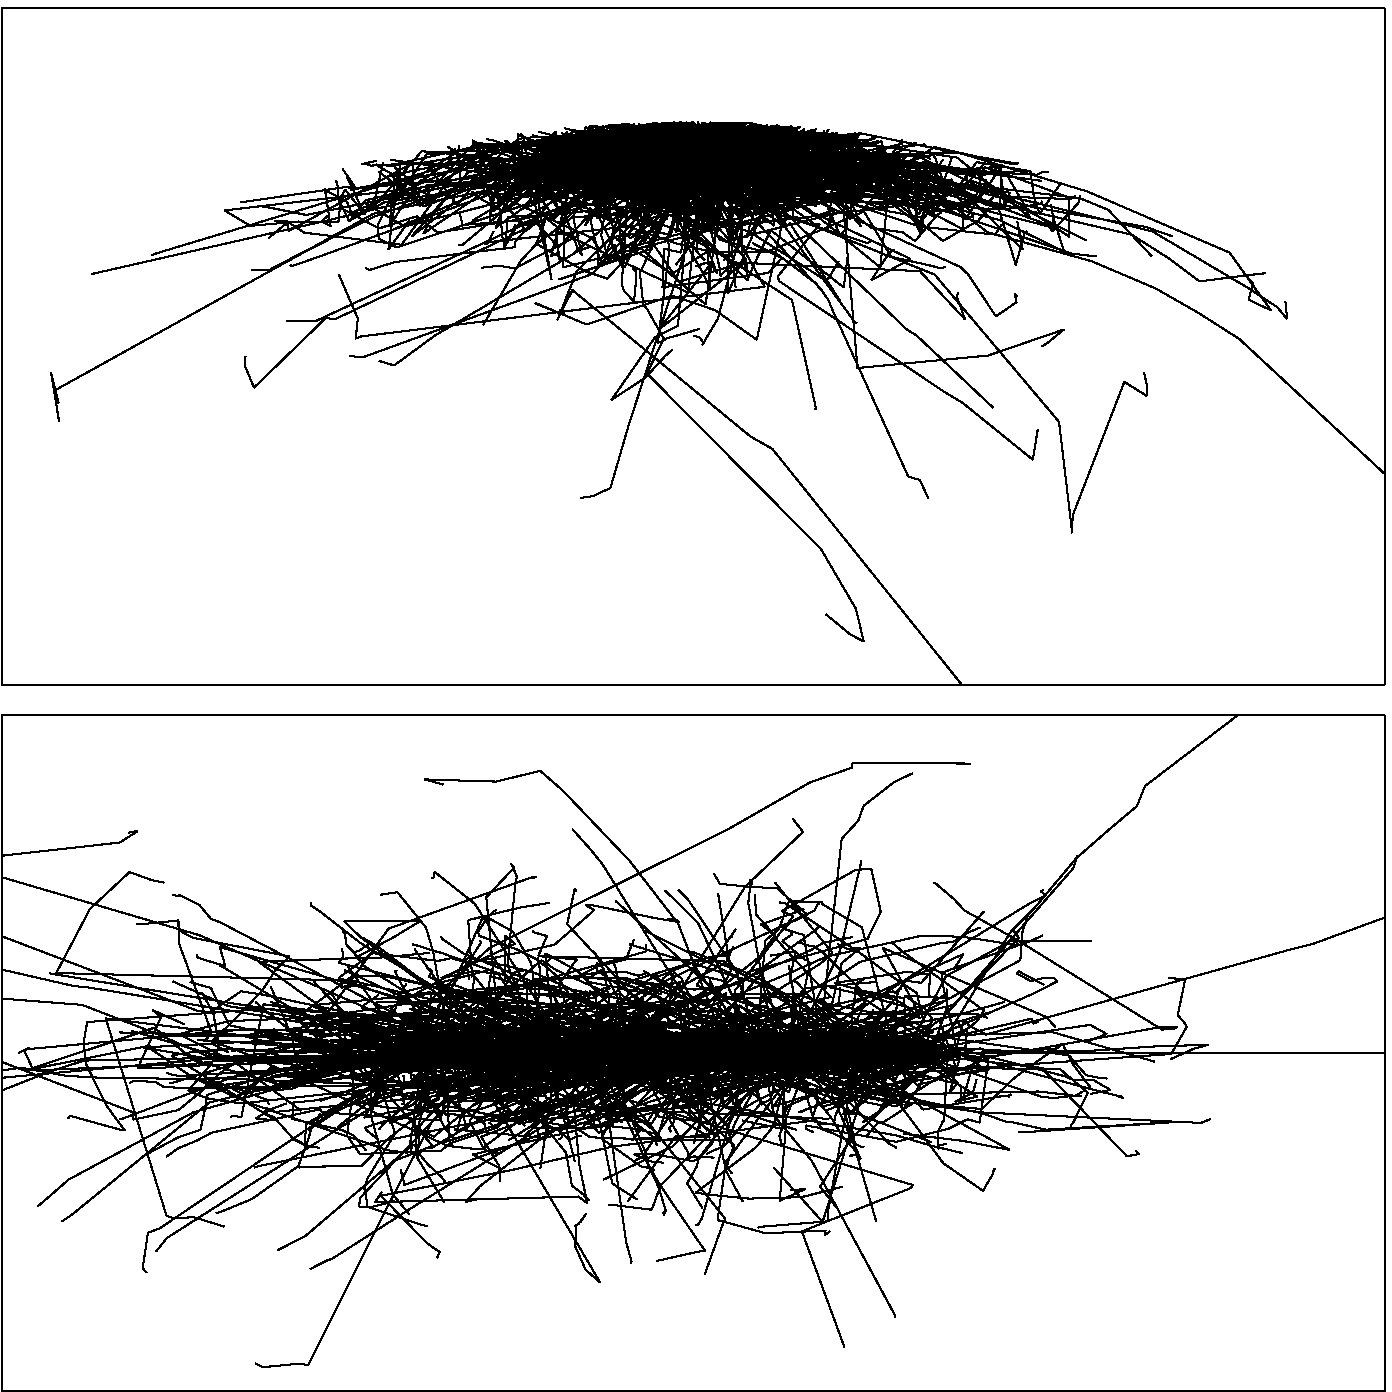
\includegraphics[width=0.6\textwidth]{images/sirotraje.pdf}
    \caption{Siro simulation of the photon paths in the atmosphere in limb-viewing geometry. Upper panel: view from the instrument. Lower panel: view from above. 
      The simulation was run for the 30~km tangent height using 1000 photons.}
    \label{siro_trajectories}
\end{figure}
